%*******************************************************************************
%****************************** Second Chapter *********************************
%*******************************************************************************

\chapter{IoT và Các kiến thức cơ bản}

\ifpdf
    \graphicspath{{Chapter2/Figs/Raster/}{Chapter2/Figs/PDF/}{Chapter2/Figs/}}
\else
    \graphicspath{{Chapter2/Figs/Vector/}{Chapter2/Figs/}}
\fi


%\section[Short title]{Reasonably long section title}
\section{Giới thiệu về Internet of Things và các ứng dụng giám sát}
\subsection{Internet of Things (IoT)}
Với sự phát triển nhanh chóng của công nghê máy tính hiện nay, những công nghệ cao đã đang và ngày càng được ứng dụng trong nhiều lĩnh vực của cuộc sống con người. IoT là mạng lưới của các đối tượng vật lý, các thiết bị, các phương tiện và các đối tượng này được nhúng với các thiết bị điện tử, cảm biến, phần mềm điều khiển, và nó có khả năng trao đổi dữ liệu và thao tác với nhau. IoT cho phép các đối tượng được lắng nghe và điều khiển từ xa trên cơ sở hạ tầng mạng hiện có, các hệ thống máy tính có thể thu thập dữ liệu và điều khiển các thiết bị đối tượng một cách hiệu quả, chính xác và lợi ích kinh tế nhất có thể. 
\begin{figure}[htbp!] 
\centering    
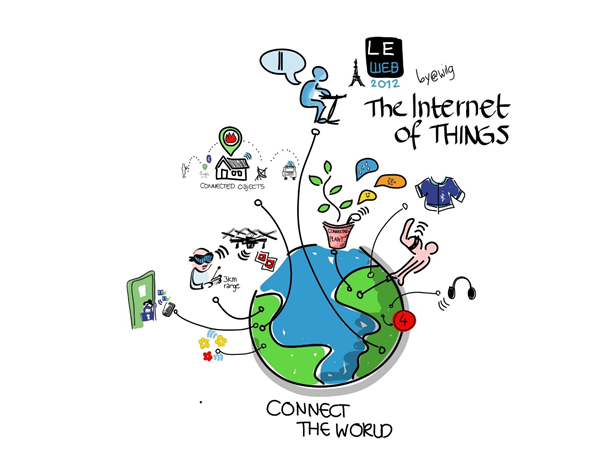
\includegraphics[width=1.0\textwidth]{pic4}
\caption[Hình ảnh mô tả Internet of Things ]{Hình ảnh mô tả Internet of Things }
\label{fig:pic4}
\end{figure}


\subsection*{Khả năng định danh độc nhất }
Điểm quan trọng của IoT đó là các đối tượng phải có thể được nhận biết và định dạng. Nếu mọi đội tượng, kể cả con người, được "đánh dấu" để phân biệt bản thân đối tượng đó với những thứ xung quanh thì chúng ta có thể hoàn toàn quản lí được nó thông qua máy tính. Việc đánh dấu có thể được thực hiện thông qua nhiều công nghệ, chẳng hạn như RFID, NFC, mã vạch, mã QR, watermark kĩ thuật số... Việc kết nối thì có thể thực hiện qua Wi-Fi, mạng viễn thông băng rộng (3G, 4G), Bluetooth, ZigBee, hồng ngoại...
Ngoài những kĩ thuật nói trên, nếu nhìn từ thế giới web, chúng ta có thể sử dụng các địa chỉ độc nhất để xác định từng vật, chẳng hạn như địa chỉ IP. Mỗi thiết bị sẽ có một IP riêng biệt không nhầm lẫn. Sự xuất hiện của IPv6 với không gian địa chỉ cực kì rộng lớn sẽ giúp mọi thứ có thể dễ dàng kết nối vào Internet cũng như kết nối với nhau.

\subsection*{Xu hướng và tính chất của The Internet of Things }
\textbf{Thông minh:} Sự thông minh và tự động trong điều khiển thực chất không phải là một phần trong ý tưởng về IoT. Các máy móc có thể dễ dàng nhận biết và phản hồi lại môi trường xung quanh (ambient intelligence), chúng cũng có thể tự điều khiển bản thân (autonomous control) mà không cần đến kết nối mạng. Tuy nhiên, trong thời gian gần đây người ta bắt đầu nghiên cứu kết hợp hai khái niệm IoT và autonomous control lại với nhau. Tương lai của IoT có thể là một mạng lưới các thực thể thông minh có khả năng tự tổ chức và hoạt động riêng lẻ tùy theo tình huống, môi trường, đồng thời chúng cũng có thể liên lạc với nhau để trao đổi thông tin, dữ liệu.

Việc tích hợp trí thông minh vào IoT còn có thể giúp các thiết bị, máy móc, phần mềm thu thập và phân tích các dấu vết điện tử của con người khi chúng ta tương tác với những thứ thông minh, từ đó phát hiện ra các tri thức mới liên quan tới cuộc sống, môi trường, các mối tương tác xã hội cũng như hành vi con người.

\textbf{Kiến trúc dựa trên sự kiện:} Các thực thể, máy móc trong IoT sẽ phản hồi dựa theo các sự kiện diễn ra trong lúc chúng hoạt động theo thời gian thực. Một số nhà nghiên cứu từng nói rằng một mạng lưới các sensor chính là một thành phần đơn giản của IoT.

\textbf{Là một hệ thống phức tạp:}Trong một thế giới mở, IoT sẽ mang tính chất phức tạp bởi nó bao gồm một lượng lớn các đường liên kết giữa những thiết bị, máy móc, dịch vụ với nhau, ngoài ra còn bởi khả năng thêm vào các nhân tốc mới.

\textbf{Kích thước: } Một mạng lưới IoT có thể chứa đến 50 đến 100 nghìn tỉ đối tượng được kết nối và mạng lưới này có thể theo dõi sự di chuyển của từng đối tượng. Một con người sống trong thành thị có thể bị bao bọc xung quanh bởi 1000 đến 5000 đối tượng có khả năng theo dõi.

\textbf{Vấn đề không gian, thời gian: }Trong IoT, vị trí địa lý chính xác của một vật nào đó là rất quan trọng. Hiện nay, Internet chủ yếu được sử dụng để quản lí thông tin được xử lý bởi con người. Do đó những thông tin như địa điểm, thời gian, không gian của đối tượng không mấy quan trọng bởi người xử lí thông tin có thể quyết định các thông tin này có cần thiết hay không, và nếu cần thì họ có thể bổ sung thêm. Trong khi đó, IoT về lý thuyết sẽ thu thập rất nhiều dữ liệu, trong đó có thể có dữ liệu thừa về địa điểm, và việc xử lí dữ liệu đó được xem như không hiệu quả. Ngoài ra, việc xử lí một khối lượng lớn dữ liệu trong thời gian ngắn đủ để đáp ứng cho hoạt động của các đối tượng cũng là một thác thức hiện nay.

\newpage

\subsection*{Mô hình theo xu hướng IoT thực tế}
Mô hình (Hình ~\ref{fig:pic5}): Các thiết bị sẽ có thể kết nối với nhau bằng TCP/UDP và có thể kết nối trực tiếp đến máy chủ mà không cần thông qua thiết bị khác.

\begin{figure}[htbp!] 
\centering    
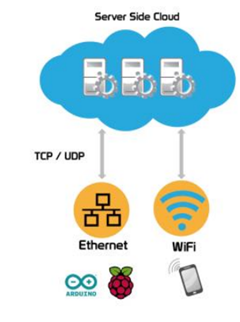
\includegraphics[width=0.5\textwidth]{pic5}
\caption[Mô hình IoT không có Gateway ]{Mô hình IoT không có Gateway}
\label{fig:pic5}
\end{figure}

Mô hình (Hình ~\ref{fig:pic6}): Các thiết bị sẽ được hỗ trợ nhiều chuẩn giao tiếp khác nhau (BLE, ZWave,…) nên cần cầu nối là Gateway để kết nối đến máy chủ. 
	
	

\begin{figure}[htbp!] 
\centering    
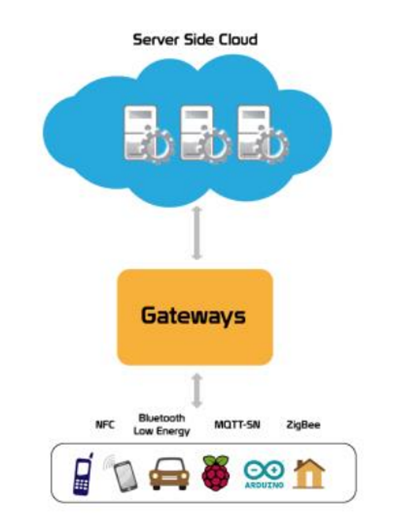
\includegraphics[width=0.5\textwidth]{pic6}
\caption[Mô hình IoT có Gateway]{Mô hình IoT có Gateway}
\label{fig:pic6}
\end{figure}


Sơ đồ lớp Chung của cả hai mô hình trên:


\begin{figure}[htbp!] 
\centering    
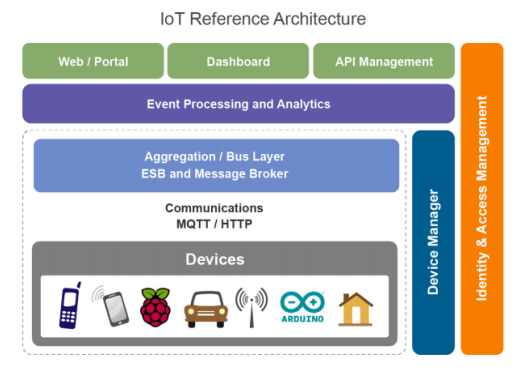
\includegraphics[width=1\textwidth]{pic7}
\caption[Kiến trúc mô hình IoT tham khảo]{Kiến trúc mô hình IoT tham khảo}
\label{fig:pic7}
\end{figure}



\begin{itemize}
\item[•]Lớp Device \\
Lớp dưới cùng của kiến trúc là lớp thiết bị. Thiết bị có thể được các loại khác nhau, nhưng để có thể được xem là thiết bị IOT, nó phải có một số thông tin liên lạc hoặc gián tiếp hoặc trực tiếp với Internet.\\
Mỗi thiết bị thường cần một ID. ID có thể là: Bluetooth identifier, Wi-Fi MAC Address…
\item[•]Lớp Communications \\
Các lớp truyền thông hỗ trợ các kết nối của các thiết bị tới máy chủ. Có nhiều giao thức để giao tiếp giữa các thiết bị và máy chủ. Nổi bật nhất là HTTP hoặc MQTT.\\
HTTP rất thông dụng. Bởi vì nó là một giao thức dựa trên văn bản đơn giản, nhiều thiết bị nhỏ như bộ điều khiển 8-bit có thể hỗ trợ một phần các giao thức - ví dụ đủ dữ liệu để POST hoặc GET một nguồn tài nguyên. Các thiết bị lớn hơn 32-bit có thể sử dụng đầy đủ các thư viện HTTP client đúng cách để hiện thực toàn bộ giao thức.\\
MQTT được phát minh vào năm 1999 để giải quyết các vấn đề trong hệ thống nhúng và SCADA. Nó đã được thông qua một số lần lặp lại và phiên bản hiện tại (3.1.1) đang trải qua những tiêu chuẩn hoá trong OASIS MQTT kỹ thuật Committee8. MQTT là một hệ thống tin nhắn publish-subscribe dựa trên một mô hình broker. Các giao thức có một chi phí rất nhỏ (ít nhất là 2 byte cho mỗi tin nhắn). MQTT được thiết kế để vận hành qua TCP.

\item[•]Lớp Aggregation/Bus \\
Một lớp quan trọng của kiến trúc là lớp mà tập hợp và là cầu nối, có khả năng tổng hợp và kết hợp các thông tin liên lạc từ các thiết bị khác nhau và đưa thông tin liên lạc đến một thiết bị cụ thể (có thể thông qua một gateway).
\item[•]Lớp Event Processing and Analytic: \\
Lớp này có các sự kiện từ lớp Bus và cung cấp khả năng xử lý và hành động theo những sự kiện này. Yêu cầu phải lưu trữ các dữ liệu vào một cơ sở dữ liệu nên buộc phải có một ứng dụng ở máy chủ.
\item[•]Lớp External Communications (Top) \\
Lớp này cung cấp một cách cho các thiết bị để chúng giao tiếp ra bên ngoài hệ thống một cách có định hướng và thân thiện với người dùng (Web, Dashboard, API Management)
\end{itemize}

% Please add the following required packages to your document preamble:

\begin{table}[]
\centering
\caption{My caption}
\label{my-label}
\begin{tabular}{|l|l|l|}
\hline
\textbf{MÔ HÌNH} & \textbf{ƯU ĐIỂM} & \textbf{NHƯỢC ĐIỂM} \\ \hline
\textbf{Mô hình cũ} & Đơn giản hiện thực & \begin{tabular}[c]{@{}l@{}}Gateway cồng kềnh vì phải có \\ bộ phận thu/phát hồng ngoại \\ và các mạch để giao tiếp RF.\end{tabular} \\ \hline
\textbf{Mô hình 1} & \begin{tabular}[c]{@{}l@{}}Không cần thông qua \\ gateway, mọi thông tin \\ thiết bị đều được lưu \\ trên máy chủ.\end{tabular} & \begin{tabular}[c]{@{}l@{}}Hạn chế về phương thức giao\\ tiếp vì chỉ sử dụng TCP/UDP \\ để giao tiếp. Không thể điều khiển\\  thiết bị khi không truy cập được \\ máy chủ.\end{tabular} \\ \hline
\textbf{Mô hình 2} & \begin{tabular}[c]{@{}l@{}}Quản lý thiết bị thông qua\\ gateway làm trung gian, nên\\ các thiết bị có thể tương tác\\ với nhau dễ dàng mà không \\ cần đến máy chủ.\end{tabular} & \begin{tabular}[c]{@{}l@{}}Chi phí cao hơn, hệ thống \\ phức tạp hơn. Độ bảo mật \\ cũng cần được quan tâm hơn.\end{tabular} \\ \hline
\end{tabular}
\end{table}



	
\subsection{Các hệ thống giám sát được phát triển dựa trên IoT}
Khi kết nối một chuỗi khổng lồ các cảm biến (sensor) thu thập dữ liệu, thiết bị và máy móc với nhau, điều quan trọng cần nhận ra là thông tin sẽ được chuyển đổi thành hành động với một tốc độ mà chúng ta chưa từng thấy trước kia. Chúng ta đang tiến đến gần, nếu không phải là đã chạm được vào một thế giới của những khoảng thời gian phản ứng cực nhỏ, phản hồi tức thì với mọi điều kiện biến đổi, và mức độ điều khiển chưa từng có trong việc quản lý tài nguyên và tài sản.
Điểm mấu chốt ở đây là đừng nghĩ hẹp. Internet of Things (IoT) không đơn thuần là mang đến sự tiết kiệm trong các mô hình công nghiệp hiện tại. Nó đảo lộn hoàn toàn những mô hình cũ, tạo ra những sản phẩm và dịch vụ mới. Không có một lĩnh vực nào mà trong đó IoT tạo ra ảnh hưởng đặc biệt lớn nhất; bởi IoT sẽ thay đổi hoàn toàn mọi lĩnh vực một cách không thể tưởng tượng được, bao gồm nông nghiệp, năng lượng, an ninh, quản lý thảm họa, y tế, và đó chỉ là một vài lĩnh vực được nhắc đến.

\subsection*{Ứng dụng trong xây dụng }
\begin{figure}[htbp!] 
\centering    
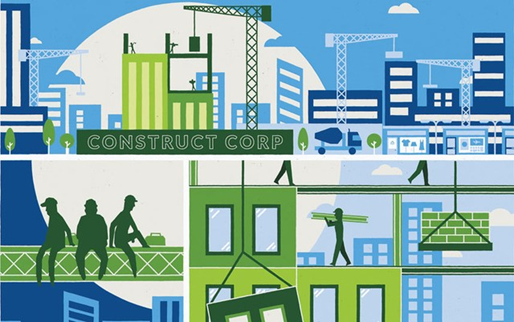
\includegraphics[width=1\textwidth]{pic8}
\caption[Ứng dụng IoT trong xây dựng ]{Ứng dụng IoT trong xây dựng }
\label{fig:pic8}
\end{figure}

Ví dụ: Các công ty xây dựng đã bắt đầu trang bị các silo (hầm chứa đồ) và xe tải có các cảm biến theo dõi mức hàng tồn kho, như là lượng bê tông, và biến đổi nó thông qua platform trên nền điện toán đám mây để gia tăng tốc độ phân phối và đảm bảo một dòng lưu thông vật liệu ổn định. Các ông lớn trong ngành công nghiệp dầu mỏ đã bắt đầu thực thi các công nghệ mobile, cảm biến tới máy móc để dự phòng từ trước cho các tai nạn thông qua các phân tích nhanh chóng và hành động tức thời. Khi các cảm biến phát hiện ra một sự cố như rò rỉ hoặc thất thoát đường ống, công nghệ IoT cho phép các công nhân lập tức xác định vị trí của chúng.

\subsection*{Ứng dụng trong năng lượng }

\begin{figure}[htbp!] 
\centering    
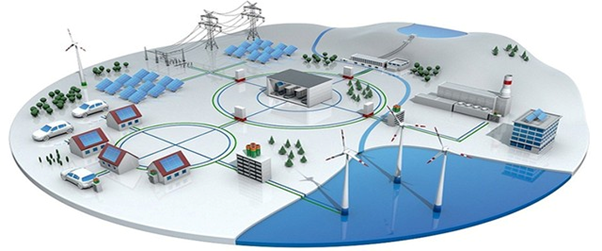
\includegraphics[width=1\textwidth]{pic9}
\caption[Ứng dụng IoT trong năng lượng]{Ứng dụng IoT trongnăng lượng}
\label{fig:pic9}
\end{figure}
Một ví dụ khác của công nghệ IoT mới ứng dụng trong công nghiệp dầu mỏ, đó là giếng thông minh. Đây là một dạng giếng cài đặt các thiết bị điều khiển dòng chảy và cảm biến lỗ khoan, để có thể giám sát và điều khiển từ trên bề mặt mà không đe dọa an toàn của công nhân. Giếng thông minh có trang bị công nghệ địa chấn 4D, cho phép theo dõi sự rò rỉ khí ga, dòng chảy nước, thay đổi áp lực, và bất cứ thay đổi nào khác gây ra bởi những biến động địa chấn, giúp cho việc dự đoán và điều khiển các tác động địa chấn có thể gây ra những hỏng hóc nghiêm trọng.
Nhưng như thế, chúng ta vẫn nghĩ quá hẹp. Hãy vượt ra khỏi lĩnh vực xây dựng hay năng lượng. Chúng ta có các cảm biến có thể đo lực, tải, moment, và áp lực; các cảm biến có thể ngửi thấy mùi khí ga hay hóa chất; những cảm biến có thể nghe thấy rung động và phân biệt giữa các âm hưởng khác nhau; những cảm biến có thể đo nhiệt độ, phát hiện chuyển động, vận tốc và chuyển vị; xác định vị trí, sự có mặt, và khoảng cách. Nói cách khác, chúng ta có khả năng thu thập những hiểu biết gần như không giới hạn, trong thời gian thực.

\subsection*{Ứng dụng trong dân dụng  }

\begin{figure}[htbp!] 
\centering    
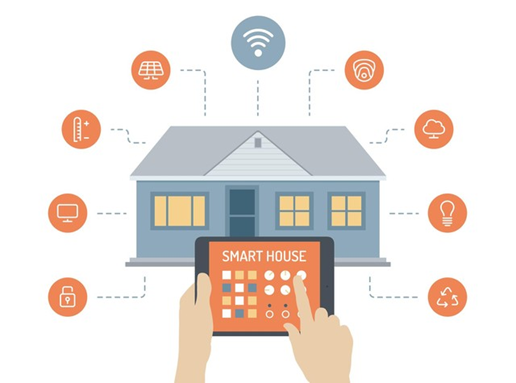
\includegraphics[width=1\textwidth]{pic10}
\caption[Ứng dụng IoT trong dân dụng ]{Ứng dụng IoT trong dân dụng}
\label{fig:pic10}
\end{figure}

Làm thế nào chúng ta có thể tận dụng thông tin thời gian thực từ rất nhiều sensor? Hãy nhìn vào ngôi nhà của chúng ta. Những phần nào trong đó có thể thông minh hóa? Ví dụ đơn giản. Tôi từng quan sát 1 hệ thống video conference cho phép người chủ nói chuyện với chú cún của mình, gọi nó đến, cho nó ăn từ xa thông qua một thiết bị thông minh. Hãy nghĩ lớn hơn nữa. Một ngôi nhà biết khi nào bạn về nhà bởi nó kết nối với một cảm biến trên xe hay smartphone của bạn. Một ngôi nhà kết nối các cảm biến báo khói, hệ thống an ninh, và thiết bị giải trí tới điện thoại của bạn. Một ngôi nhà với các cảm biến được gắn vào đường ống để có thể phát hiện ra rò rỉ trước cả khi điều đó thực sự diễn ra.

\subsection*{Ứng dụng trong y tế}
\begin{figure}[htbp!] 
\centering    
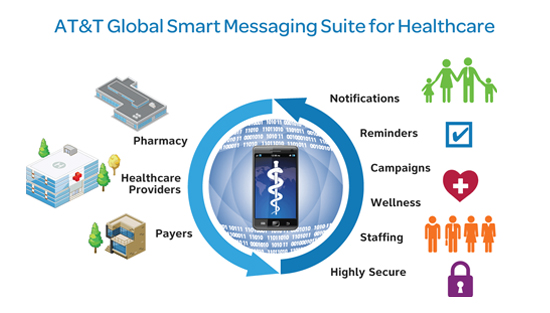
\includegraphics[width=1\textwidth]{pic11}
\caption[Ứng dụng IoT trong y tế ]{Ứng dụng IoT trong y tế}
\label{fig:pic11}
\end{figure}
Công nghệ thiết bị đeo cũng sẽ biến đổi hoàn toàn lĩnh vực chăm sóc sức khỏe theo những cách phi thường. Chúng ta đều biết rằng đồng hộ Apple Watch sẽ tích hợp một cảm biến theo dõi nhịp tim và cung cấp cho chủ của nó những ứng dụng tạo điều kiện và khuyến khích một cách sống lành mạnh. Chúng ta đã có các cảm biến gắn trong giày để theo dõi việc chạy xa đến đâu và bao nhiêu calo đã được đốt. Còn gì tiếp theo? Sẽ có một quy trình tối ưu chăm sóc sức khỏe, theo đó có những cảm biến có thể phát hiện vi khuẩn trong thiết bị, và thiết bị diệt khuẩn phát hiện virus có thể di chuyển từ bệnh nhân.


\section{Giới thiệu về các công cụ hỗ trợ phát triển ứng dụng IoT}




\section{Những yếu tố ảnh hưởng môi trường từ khí thải phương tiện giao thông}
Để hình dung được những yếu tố ảnh hưởng môi trường từ khí thải xe máy và ô tô thì chúng ta cần biết được quá trình hoạt động của xe máy và ô tô, từ đó chúng ta sẽ biết được những loại khí thải nào mà xe máy và ô tô sẽ thải ra môi trường. Qua quá trình tìm hiểu và đọc thông tin tài liệu trên mạng khí thải của xe máy và ô tô tuỳ thuộc chủ yếu vào chất lượng đốt cháy hỗn hợp xăng và không khí bên trong buồng đốt (combustion chamber) của động cơ, cũng như nồng độ các chất ô nhiễm trong khí xả phụ thuộc vào đặc điểm động cơ cũng như các thông số điều chỉnh, vận hành.

Động cơ mới và được điều chỉnh đúng cho phản ứng cháy hoàn chỉnh (complete combustion) hay phản ứng cháy thừa oxy:

\begin{center}
PTPU: Xăng + Không khí → Carbon Dioxide + Nước + Nitrogen
\end{center} 
Các phó sản (by-product) chủ yếu của phản ứng này là nước (H2O) và carbon dioxide (CO2), do đó ống thoát khí cháy (tail pipe) của một động cơ tốt thường có nước nhễu ra, dễ nhận thấy khi động cơ đang trong quá trình làm nóng máy (warm up).
Động cơ cũ hoặc không được điều chỉnh đúng cho phản ứng cháy không hoàn chỉnh (incomplete combustion) hay thiếu oxy:
\begin{center}
PTPU: Xăng + Không khí → Hydrocarbons + Nitrogen Oxides + Carbon Dioxide + Carbon Monoxide + Nước
\end{center}

Phản ứng này tạo thêm những phó sản như carbon monoxide (CO) và nitrogen oxides (NOx). Vậy chúng ta có các loại sản pham như sau:
\begin{itemize}
\item[•]CO được sinh ra khi lượng oxy đưa vào buồng đốt không đủ.
\item[•]HC được sinh ra trong quá trình đốt cháy không hoàn toàn, cũng như CO.
\item[•]NOx được sinh ra do nitơ và ôxy trong hỗn hợp không khí-nhiên liệu, khi nhiệt độ của buồng đốt tăng cao trên 1800oC.
\end{itemize}
 Nhiệt độ của buồng đốt càng cao, lượng NOx sản ra càng nhiều.
Theo lý thuyết, khi đốt cháy xăng thì chỉ sinh ra CO2 (cácbon điôxit) và H2O (hơi nước). Tuy nhiên, không phải toàn bộ xăng đều tham gia phản ứng như lí thuyết, do ảnh hưởng của các yếu tố như tỷ lệ hỗn hợp không khí-nhiên liệu, nitơ trong không khí, nhiệt độ cháy, thời gian cháy... Đó là nguyên nhân sinh ra các khí độc hại như CO, HC hoặc NOx.
Trên cơ sở thực tế, động cơ đốt trong nó chỉ sử dụng được khoảng 30-45\% nhiệt lượng để sinh công, phần còn lại bị hao hụt đi mất, do đó nó mang theo nhiệt lượng thải ra ngoài. Lượng nhiệt này thực tế đã tác động đến môi trường, làm cho nhiệt độ xung quanh những khu vực có xe máy và ô tô tăng lên. Việc đi lại trên những đoạn đường đông xe máy và ô tô thường gây cho chúng ta cảm giác nóng bức, và khó thở. Đó chính là những yếu tố khí thải đã trình bày như trên của xe máy và ô tô đã tác động đến môi trường.
Một phần nhân tố cũng đáng chú ý trong quá trình hoạt động xe máy và ô tô hoạt động đó là bụi, vì đầu vào của động cơ là xăng và không khí, mà trong xăng hiện nay thường có cặn và lượng không khí đầu vào cũng có bụi mặc dù có bộ lọc khí nhưng không thể tránh được trong quá trình sử dụng lâu dài. Một số loại phương tiện giao thông sử dụng thời gian dài, không đi bảo trì sẽ thải ra một nồng độ ô nhiễm rất lớn.
Từ những cơ sơ lý thuyết trên cho chúng ta biết được những yếu tố ảnh hưởng môi trường từ khí thải xe máy và ô tô bao gồm:
\begin{itemize}
\item[•]Khí CO2, CO, HC, NOx.
\item[•]Khói bụi.
\item[•]Yếu tố về nhiệt.
\end{itemize}








\section{Các hệ thống quan trắc hiện hữu}
\textbf{VoV giao thông:}  sử dụng hệ thống camera an ninh kết hợp với lượng phóng viên thường trực khắp thành phố để giám sát trực tiếp và cảnh báo tình trạng lưu thông trên các đoạn đường. Hệ thống có tính hiệu quả rất cao vì sử dụng CCTV giám sát tình trạng giao thông theo thời gian thực nên có góc nhìn thực tế nhất và không phục thuộc, có thể hoạt động độc lập. Tuy nhiên hệ thống vẫn có nhiều hạn chế như:
\begin{itemize}
\item[•]Vẫn chủ yếu hoạt động một cách thủ công, điều tiết và đưa ra kết quả bởi con người, chưa có áp dụng thuật toán xử lý máy tính vào công việc nhiều.
\item[•]Tốn nhiều công sức và nhân lực, cần có nhiều phóng viên trực thuộc các đoạn đường cũng như người quản lý theo dõi hệ thống camera giao thông.
\item[•]Chi phí duy trì và lắp đặt còn khá cao, và cần tốn chi phí bảo trì đắt đỏ và trình độ chuyên môn nhân viên điều hành cao, chi phí một hệ thống có thể lên tới hàng trăm tỉ. Cụ thể như hệ thống trị giá 270 tỉ VNĐ bao gồm 19 trạm giám sát camera được triển khai ở Bà Rịa - Vũng Tàu.
\end{itemize}

\begin{figure}[htbp!] 
\centering    
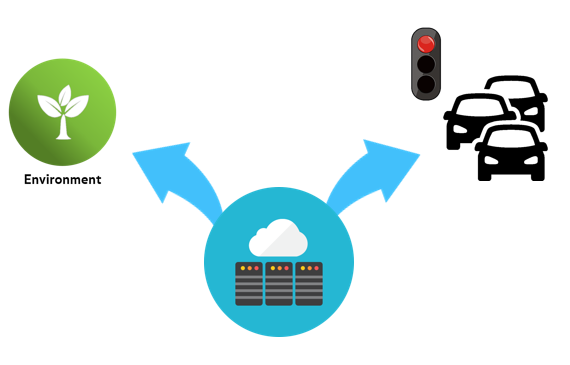
\includegraphics[width=1.0\textwidth]{pic1}
\caption[Trạm giám sát VOV Giao thông ]{Trạm giám sát VOV Giao thông}
\label{fig:pic1}
\end{figure}




\textbf{Bktraffic}  \url{http://traffic.hcmut.edu.vn} kết hợp hệ thống xe bus cùng với định vị GPS và gửi dữ liệu qua hạ tầng mạng 3G để theo dõi vị trí xe và tính toán tốc độ lưu thông trên đoạn đường xe đang lưu thông. Dự án này có hiệu quả cao vì hệ thống xe bus dày đặc và có thời gian hoạt động rộng. Tuy nhiên vẫn có những hạn chế như:
\begin{itemize}
\item[•]Vì chỉ giám sát trên xe bus nhưng nhiều trường hợp không hiệu quả khi áp dụng cho giao thông tại Việt Nam. Bởi vì đa số phương tiện giao thông ở Việt Nam là xe 2 bánh, do đó hệ thống bus di chuyển không phản ảnh được tình trạng lưu thông chung trên tuyến đường đó.
\item[•]Nhiều tuyến đường trên địa bàn thành phố mà xe bus vẫn chưa hoạt động, do vậy vẫn chưa có đủ dữ liệu cần thiết để.
\item[•]Mang tính phụ thuộc vào xe bus, vậy nên có sẽ có những trường hợp ảnh hưởng bởi hệ thống xe bus mà hệ thống sẽ không hoạt động hiệu quả được.
\end{itemize}

\begin{figure}[htbp!] 
\centering    
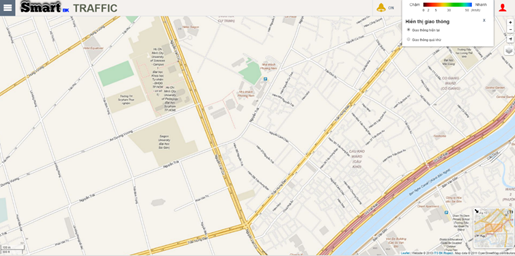
\includegraphics[width=1.0\textwidth]{pic2}
\caption[Ứng dụng Web SmartBKTraffic ]{ Ứng dụng Web SmartBKTraffic}
\label{fig:pic2}
\end{figure}




\textbf{Hệ thống quan trắc môi trường ở Hà Nội:} Thủ đô Hà Nội vừa lắp đặt hệ thống 80 trạm quan trắc. Hệ thống này có tính tương đồng với đề tài đang thực hiện. Tuy nhiên mục đích chính là để theo dõi môi trường sau sự cố bụi Thủy ngân và chưa thấy hướng ứng dụng vào hệ thống giao thông. Hơn nữa, các trạm này chiếm diện tích lắp đặt nên hạn chế khả năng triển khai số lượng lớn trên diện rộng.
\begin{figure}[htbp!] 
\centering    
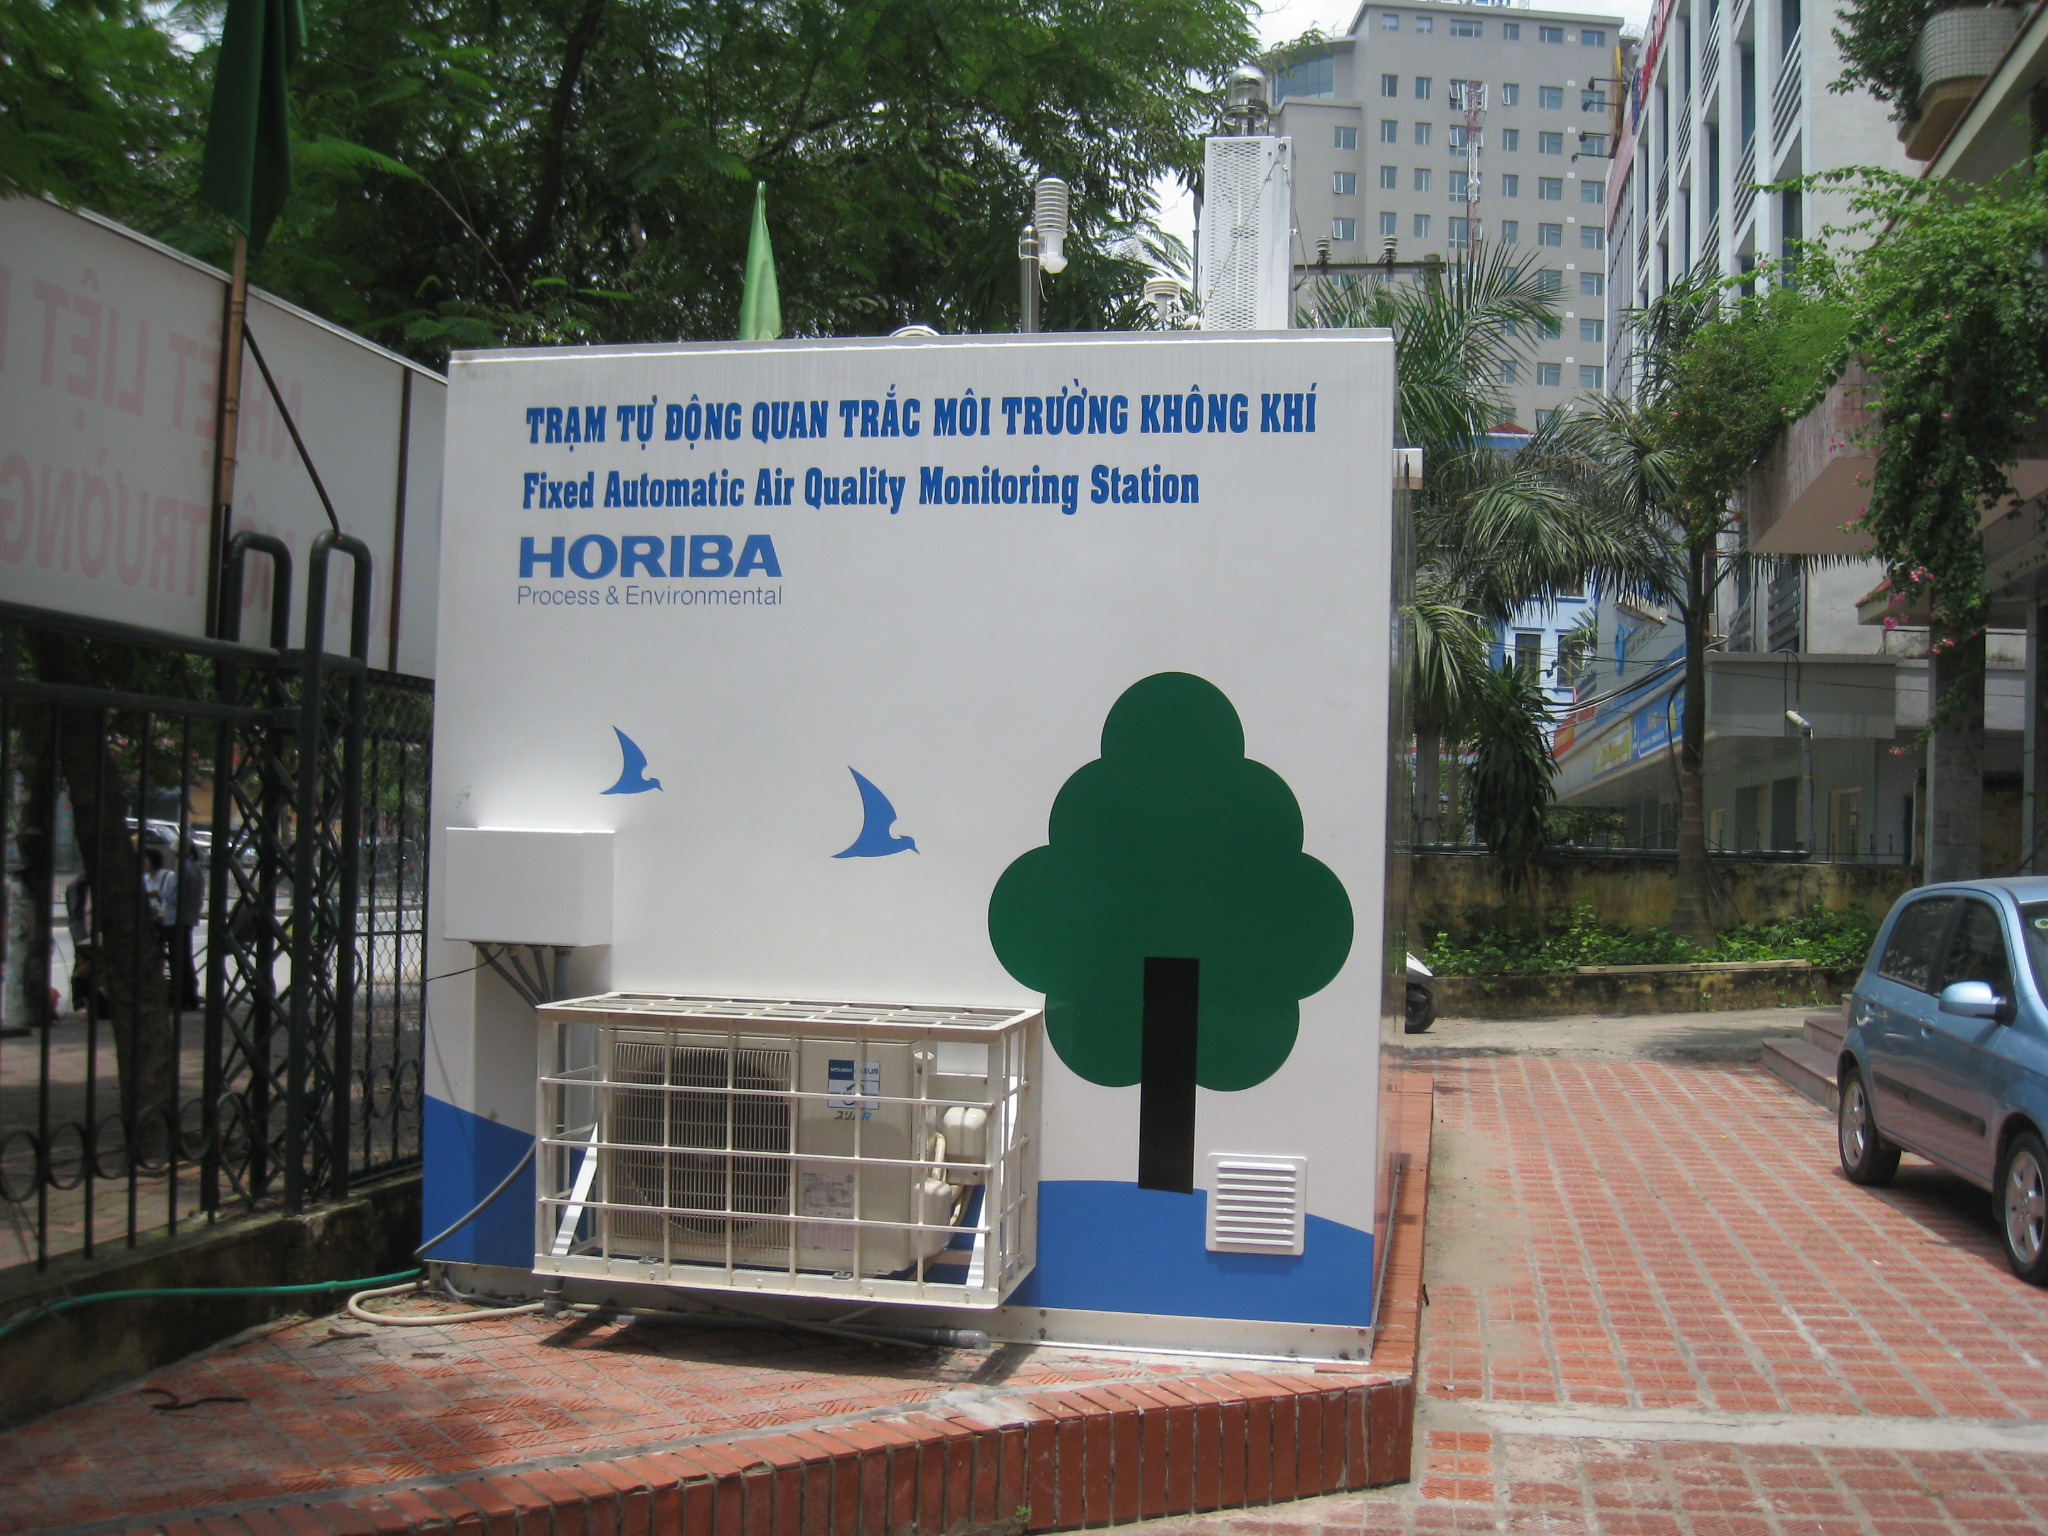
\includegraphics[width=1.0\textwidth]{pic3}
\caption[Trạm quan trắc môi trường tại Hà Nội ]{Trạm quan trắc môi trường tại Hà Nội}
\label{fig:pic3}
\end{figure}




\section*{Itemize}
\begin{itemize}
\item The first topic is dull
\item The second topic is duller
\begin{itemize}
\item The first subtopic is silly
\item The second subtopic is stupid
\end{itemize}
\item The third topic is the dullest
\end{itemize}

\section*{Description}
\begin{description}
\item[The first topic] is dull
\item[The second topic] is duller
\begin{description}
\item[The first subtopic] is silly
\item[The second subtopic] is stupid
\end{description}
\item[The third topic] is the dullest
\end{description}


\clearpage


\begin{landscape}

\section*{Subplots}
I can cite Wall-E (see Fig.~\ref{fig:WallE}) and Minions in despicable me (Fig.~\ref{fig:Minnion}) or I can cite the whole figure as Fig.~\ref{fig:animations}


\begin{figure}
  \centering
  \begin{subfigure}[b]{0.3\textwidth}
    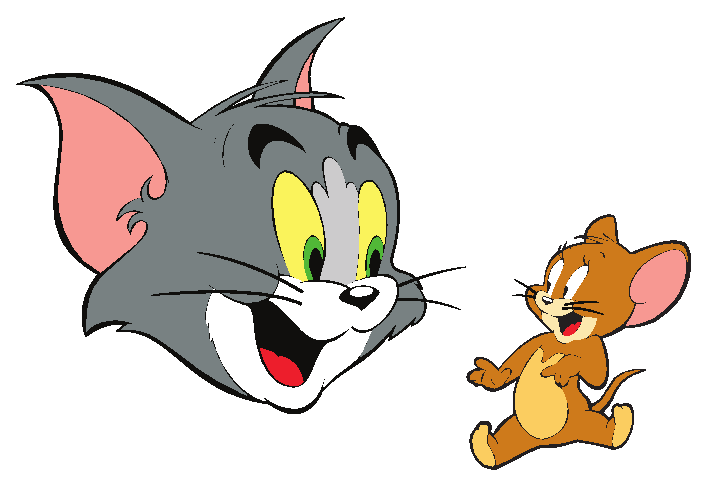
\includegraphics[width=\textwidth]{TomandJerry}
    \caption{Tom and Jerry}
    \label{fig:TomJerry}   
  \end{subfigure}             
  \begin{subfigure}[b]{0.3\textwidth}
    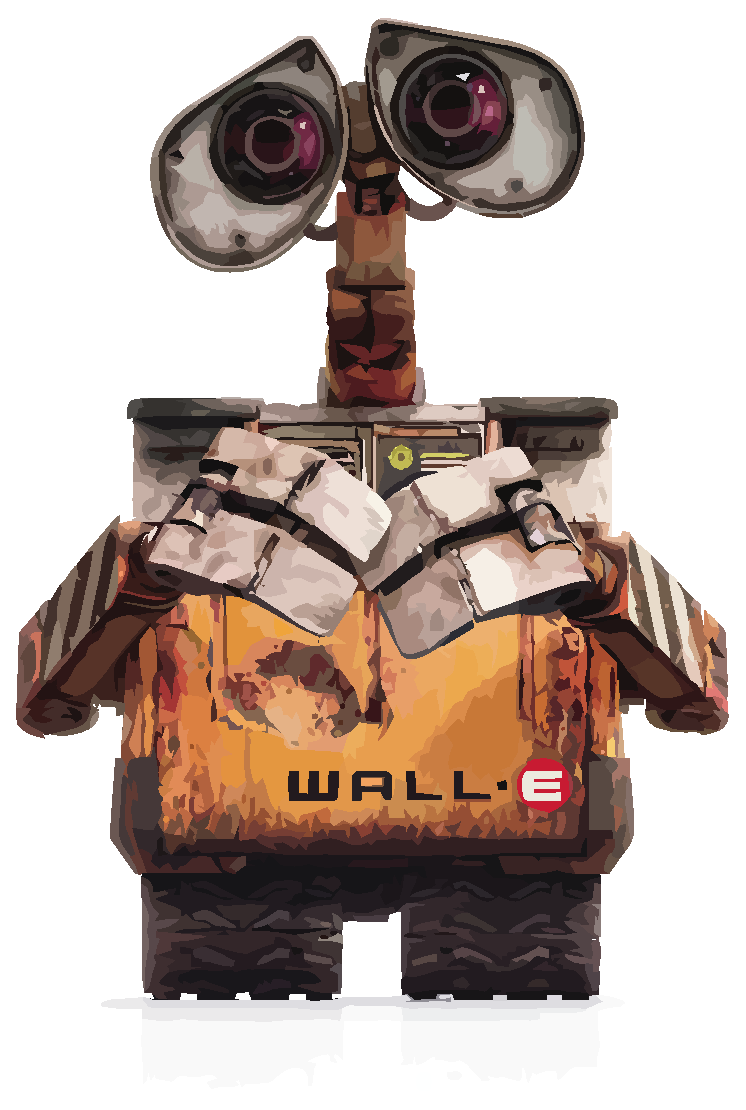
\includegraphics[width=\textwidth]{WallE}
    \caption{Wall-E}
    \label{fig:WallE}
  \end{subfigure}             
  \begin{subfigure}[b]{0.3\textwidth}
    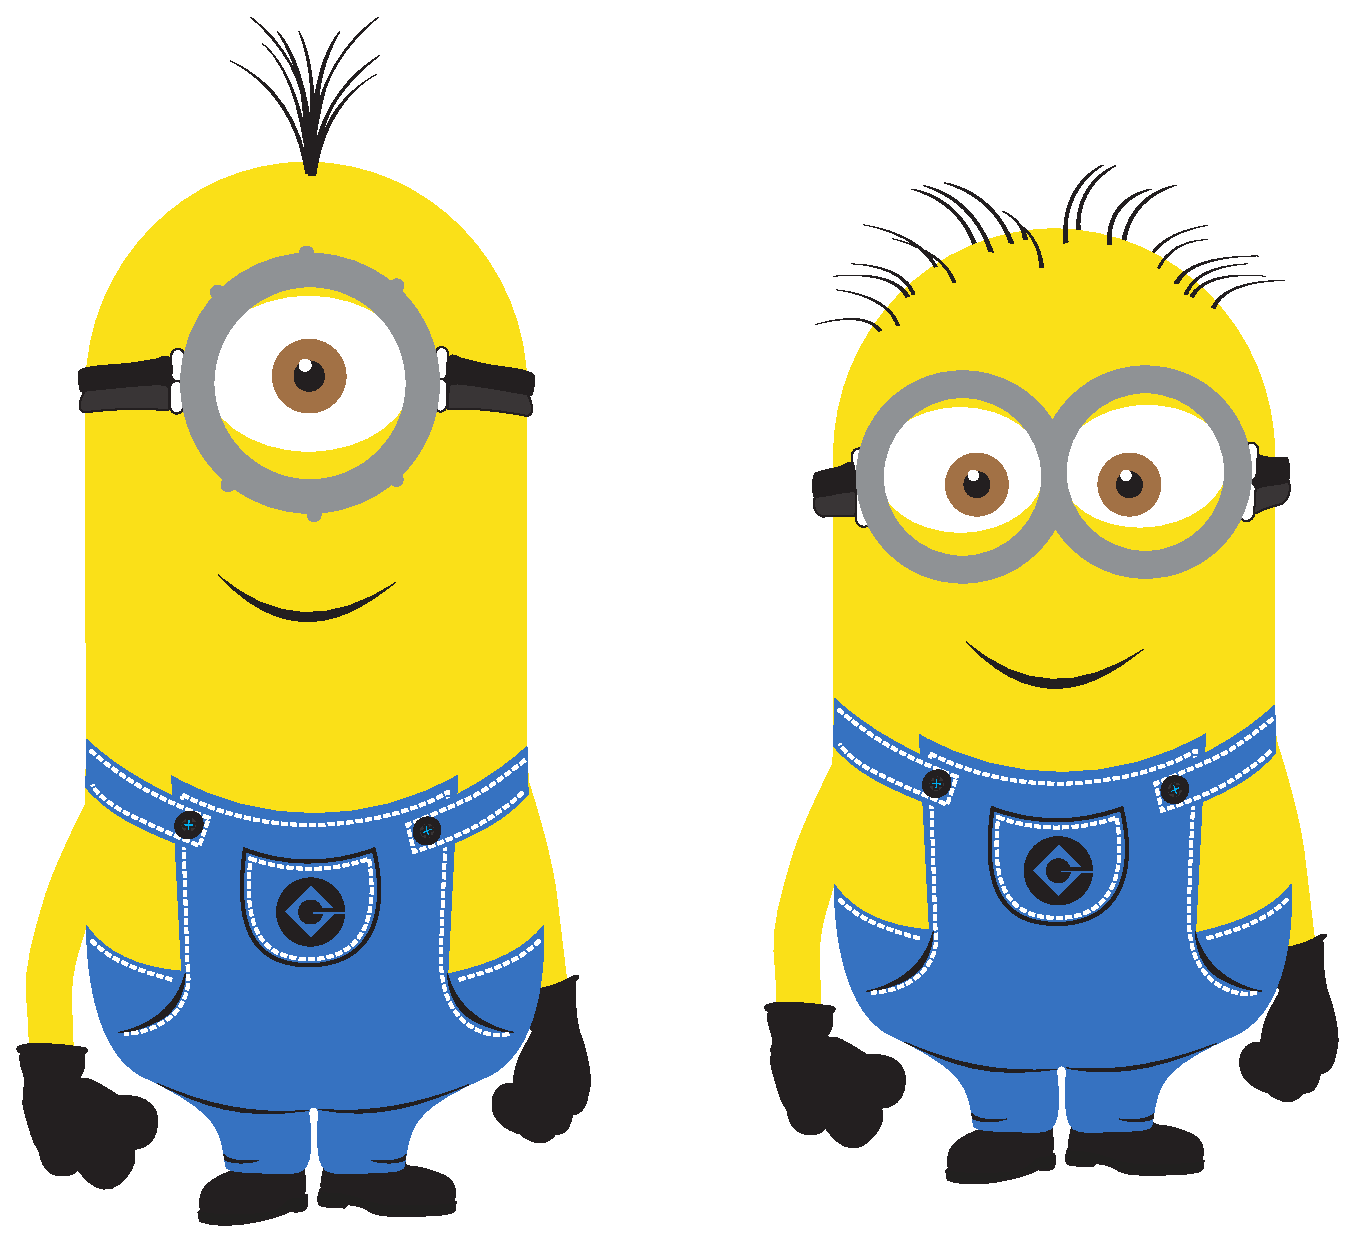
\includegraphics[width=\textwidth]{minion}
    \caption{Minions}
    \label{fig:Minnion}
  \end{subfigure}
  \caption{Best Animations}
  \label{fig:animations}
\end{figure}


\end{landscape}
